\section{根付き全域森問題のASP符号化}\label{chap:encode}

本節では,根付き全域森問題の入力と制約を論理プログラムとして表現する方
法について述べる.

%%%%%%%%%%%%%%%%%%%%%%%%%%%%%%%%%
\lstinputlisting[float=tb,caption={%
  根付き全域森問題(図~\ref{fig:dnetgraph})のファクト表現},%
captionpos=b,frame=single,label=code:graph.lp,%
xrightmargin=1zw,% 
xleftmargin=1zw,% 
numbersep=5pt,%
numbers=none,%
breaklines=true,%
columns=fullflexible,keepspaces=true,%
basicstyle=\ttfamily\scriptsize]{code/graph.lp}
%%%%%%%%%%%%%%%%%%%%%%%%%%%%%%%%%

\textbf{ASPファクト形式.} 
根付き全域森問題の入力(図~\ref{fig:dnetgraph})のファクト表現を
コード\ref{code:graph.lp}に示す.
この問題は,ノード6個,根ノード2個,辺7個から構成され,
それぞれ,アトム\code{node/1},\code{root/1},\code{edge/2}
によって表されている.
例えば,ファクト\code{edge(1,2).}は,ノード\code{1}とノード\code{2}が
隣接していることを表す.

%%%%%%%%%%%%%%%%%%%%%%%%%%%%%%%%%
\lstinputlisting[float=tb,caption={%
  根付き全域森問題の基本符号化},%
captionpos=b,frame=single,label=code:srf1.lp,%
xrightmargin=1zw,% 
xleftmargin=1zw,% 
numbersep=5pt,%
numbers=left,%
breaklines=true,%
columns=fullflexible,keepspaces=true,%
basicstyle=\ttfamily\scriptsize]{code/srf1.lp}
%%%%%%%%%%%%%%%%%%%%%%%%%%%%%%%%%
\lstinputlisting[float=tb,caption={%
  根付き全域森問題の改良符号化},%
captionpos=b,frame=single,label=code:srf2.lp,%
xrightmargin=1zw,% 
xleftmargin=1zw,% 
numbersep=5pt,%
numbers=left,%
breaklines=true,%
columns=fullflexible,keepspaces=true,%
basicstyle=\ttfamily\scriptsize]{code/srf2.lp}
%%%%%%%%%%%%%%%%%%%%%%%%%%%%%%%%%

%%%%%%%%%%%%%%%%%%%%%%%%%%%%%%%%%%%%% 
% 5節 遷移問題の解の例 (配置の関係でここに記述)
%%%%%%%%%%%%%%%%%%%%%%%%%%%%%%%%%%%%% 
\newcommand{\lw}[1]{\smash{\lower-8.ex\hbox{#1}}}
\begin{figure*}[tbp]
  %\renewcommand{\arraystretch}{0.9}
  \tabcolsep = 3mm  
  \centering
  \begin{tabular}{ccc}
    $t=0$ (スタート状態) & & $t=1$\\
    \scalebox{0.8}{%%%%%%%%%%%%%%%%%%%%%%%%%%%%%%%%%%%%%%%%%%%%%%%%%%
% 実行例(t=0) (第6章で使う)
%%%%%%%%%%%%%%%%%%%%%%%%%%%%%%%%%%%%%%%%%%%%%%%%%%

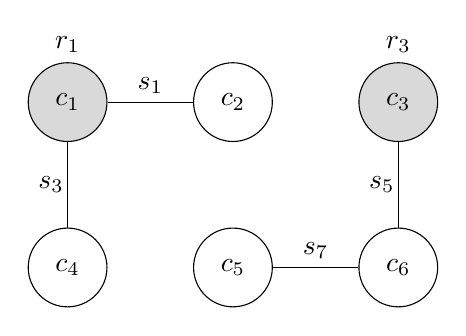
\begin{tikzpicture}[x=1.5cm,y=1.5cm,scale=0.7]

 % 設定
 \tikzset{root/.style={circle,draw=black,fill=gray!30,minimum size=1cm}}
 \tikzset{node/.style={circle,draw=black,minimum size=1cm}}
 
 % 補助線
 % \draw [help lines,blue,step=2cm] (-3,0) grid (3,-3);

 % 時間 %
 % \node[rectangle,draw=black] at (-3,1) {$t=0$};

 % root %
 \node[root] at (-2,0) (1){$c_1$};
 \node[above=0.5cm] at (1) {$r_1$};
 \node[root] at (2,0) (3){$c_3$};
 \node[above=0.5cm] at (3) {$r_3$};

 % node %
 \node[node] at (0,0) (2){$c_2$};
 \node[node] at (-2,-2) (4){$c_4$};
 \node[node] at (0,-2) (5){$c_5$};
 \node[node] at (2,-2) (6){$c_6$};

 % 繋がっていない辺は破線
 %\foreach \u / \v in {2/3, 2/5, 4/5}
 %\draw [dashed] (\u) -- (\v);
 % 繋がってる辺は実線
 \foreach \u / \v in {1/2, 1/4, 3/6, 5/6}
 \draw (\u) -- (\v);

 % スイッチ switch %
  \node at (-1,0.2) {$s_1$};
 % \node at (1,0.2) {$s_2$};
  \node at (-2.2,-1) {$s_3$};
 % \node at (-0.2,-1) {$s_4$};
  \node at (1.8,-1) {$s_5$};
 % \node at (-1,-1.8) {$s_6$};
  \node at (1,-1.8) {$s_7$};
 %

\end{tikzpicture}

%%%%%%%%%%%%%%%%%%%%%%%%%%%%%%%%%%%%%%%%%%%%%%%%%%%%%%%%%%
%%% Local Variables:
%%% mode: japanese-latex
%%% TeX-master: paper.tex
%%% End:
}
    & \lw{$\Rightarrow$} & 
    \scalebox{0.8}{%%%%%%%%%%%%%%%%%%%%%%%%%%%%%%%%%%%%%%%%%%%%%%%%%%
% 実行例(t=1) (第6章で使う)
%%%%%%%%%%%%%%%%%%%%%%%%%%%%%%%%%%%%%%%%%%%%%%%%%%

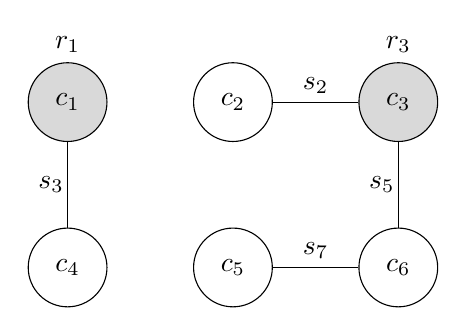
\begin{tikzpicture}[x=1.5cm,y=1.5cm,scale=0.7]

 % 設定
 \tikzset{root/.style={circle,draw=black,fill=gray!30,minimum size=1cm}}
 \tikzset{node/.style={circle,draw=black,minimum size=1cm}}
 
 % 補助線
 % \draw [help lines,blue,step=2cm] (-3,0) grid (3,-3);

 % 時間 %
 % \node[rectangle,draw=black] at (-3,1) {$t=1$};

 % root %
 \node[root] at (-2,0) (1){$c_1$};
 \node[above=0.5cm] at (1) {$r_1$};
 \node[root] at (2,0) (3){$c_3$};
 \node[above=0.5cm] at (3) {$r_3$};

 % node %
 \node[node] at (0,0) (2){$c_2$};
 \node[node] at (-2,-2) (4){$c_4$};
 \node[node] at (0,-2) (5){$c_5$};
 \node[node] at (2,-2) (6){$c_6$};

 % 繋がっていない辺は破線
 %\foreach \u / \v in {2/3, 2/5, 4/5}
 %\draw [dashed] (\u) -- (\v);
 % 繋がってる辺は実線
 \foreach \u / \v in {2/3, 1/4, 3/6, 5/6}
 \draw (\u) -- (\v);

 % スイッチ switch %
 % \node at (-1,0.2) {$s_1$};
 %
 \node at (1,0.2) {$s_2$};
 \node at (-2.2,-1) {$s_3$};
 % \node at (-0.2,-1) {$s_4$};
 \node at (1.8,-1) {$s_5$};
 % \node at (-1,-1.8) {$s_6$};
 \node at (1,-1.8) {$s_7$};
 %

\end{tikzpicture}

%%%%%%%%%%%%%%%%%%%%%%%%%%%%%%%%%%%%%%%%%%%%%%%%%%%%%%%%%%
%%% Local Variables:
%%% mode: japanese-latex
%%% TeX-master: paper.tex
%%% End:
}\\
    & & $\Downarrow$\\
    & & \\
    \scalebox{0.8}{%%%%%%%%%%%%%%%%%%%%%%%%%%%%%%%%%%%%%%%%%%%%%%%%%%
% 実行例(t=3) (第6章で使う)
%%%%%%%%%%%%%%%%%%%%%%%%%%%%%%%%%%%%%%%%%%%%%%%%%%
\begin{tikzpicture}[scale=0.6]

 % 設定
 \tikzset{node/.style={circle,draw=black,fill=white}}

 \definecolor{edge1}{RGB}{191,0,0}
 \definecolor{node1}{RGB}{249,200,200}
 \definecolor{edge3}{RGB}{38,38,134}
 \definecolor{node3}{RGB}{200,200,249}

 % 補助線
 % \draw [help lines,blue] (0,0) grid (20,6);

 % node %
 \node[circle, ultra thick, draw=edge1, fill=node1](out1){1};
 \node[node, fill=node3, right=of out1] (out2){2};
 \node[circle, ultra thick, draw=edge3,fill=node3, right=of out2](out3){3};
 \node[node, fill=node3, below=of out1] (out4){4};
 \node[node, fill=node3, below=of out2] (out5){5};
 \node[node, fill=node3, below=of out3] (out6){6};

 \foreach \u / \v in {}
 \draw [very thick, edge1] (\u) -- (\v);

 \foreach \u / \v in {out2/out3,out2/out5,out4/out5,out5/out6}
 \draw [very thick, edge3](\u) -- (\v);
\end{tikzpicture}

%%%%%%%%%%%%%%%%%%%%%%%%%%%%%%%%%%%%%%%%%%%%%%%%%%%%%%%%%%
%%% Local Variables:
%%% mode: japanese-latex
%%% TeX-master: paper.tex
%%% End:
}
    & \lw{$\Leftarrow$} &
    \scalebox{0.8}{%%%%%%%%%%%%%%%%%%%%%%%%%%%%%%%%%%%%%%%%%%%%%%%%%%
% 実行例(t=2) (第6章で使う)
%%%%%%%%%%%%%%%%%%%%%%%%%%%%%%%%%%%%%%%%%%%%%%%%%%

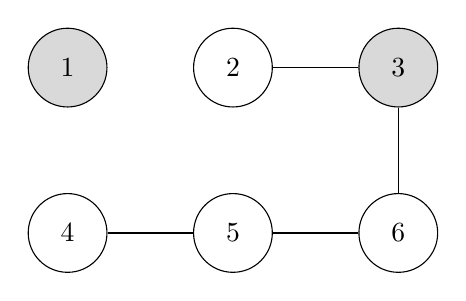
\begin{tikzpicture}[x=1.5cm,y=1.5cm,scale=0.7]

 % 設定
 \tikzset{root/.style={circle,draw=black,fill=gray!30,minimum size=1cm}}
 \tikzset{node/.style={circle,draw=black,minimum size=1cm}}
 
 % 補助線
 % \draw [help lines,blue,step=2cm] (-3,0) grid (3,-3);

 % 時間 %
 % \node[rectangle,draw=black] at (-3,1) {$t=2$};

 % root %
 \node[root] at (-2,0) (1){$1$};
% \node[above=0.5cm] at (1) {$r_1$};
 \node[root] at (2,0) (3){$3$};
 %\node[above=0.5cm] at (3) {$r_3$};

 % node %
 \node[node] at (0,0) (2){$2$};
 \node[node] at (-2,-2) (4){$4$};
 \node[node] at (0,-2) (5){$5$};
 \node[node] at (2,-2) (6){$6$};

 % 繋がっていない辺は破線
 %\foreach \u / \v in {2/3, 2/5, 4/5}
 %\draw [dashed] (\u) -- (\v);
 % 繋がってる辺は実線
 \foreach \u / \v in {2/3, 4/5, 3/6, 5/6}
 \draw (\u) -- (\v);

 % スイッチ switch %
 % \node at (-1,0.2) {$s_1$};
 % \node at (1,0.2) {$s_2$};
 % \node at (-2.2,-1) {$s_3$};
 % \node at (-0.2,-1) {$s_4$};
 % \node at (1.8,-1) {$s_5$};
 % \node at (-1,-1.8) {$s_6$};
 % \node at (1,-1.8) {$s_7$};
 %

\end{tikzpicture}

%%%%%%%%%%%%%%%%%%%%%%%%%%%%%%%%%%%%%%%%%%%%%%%%%%%%%%%%%%
%%% Local Variables:
%%% mode: japanese-latex
%%% TeX-master: paper.tex
%%% End:
}\\
    $t=3$ (ゴール状態) & & $t=2$
  \end{tabular}
  \caption{根付き全域森遷移問題 (遷移制約$d=2$) の解の一例}
  \label{fig:trans}
\end{figure*}
%%%%%%%%%%%%%%%%%%%%%%%%%%%%%%%%%%%%%

\textbf{基本符号化.}
根付き全域森問題のASP符号化をコード\ref{code:srf1.lp}に示す.
2行目のルールは,各辺(\code{X},\code{Y})に対して,
解の候補となるアトム\code{inForest(X,Y)}を導入する.
この\code{inForest(X,Y)}は,
辺(\code{X},\code{Y})が根付き全域森に含まれることを意味する.
%
各ノードの到達可能性は5~7行目のルールで表される.
アトム\code{reached(X,R)}は,ノード\code{X}は根
\code{R}から到達可能であることを意味する.
5行目のルールは,各根ノードは自分自身から到達可能であることを表す.
6~7行目のルールは,ノード\code{Y}が根ノード\code{R}から到達可能であり,
かつ,辺(\code{X},\code{Y})が全域森に含まれるならば,
ノード\code{X}も\code{R}から到達可能であることを表す.

非閉路制約は10~13行目のルールで表される.
このルールは,各連結成分のノード数と辺数の差が1になること(木の性質)を,
ASP の重み付き個数制約を使って表している.
%
根付き連結制約は16~17行目のルールで表される.
16行目のルールは,各ノードは少なくとも1つの根から到達可能であることを
表している(\textit{at-least-one}制約).
17行目のルールは,各ノードは高々1つの根から到達可能である
ことを表している(\textit{at-most-one}制約).
これら2つの一貫性制約により,各ノードはちょうど1つの根から到達可能であ
ることが強制される.

%%%%%%%%%%%%%%%%%%%%%%%%%%%%%%%%%
\textbf{改良符号化.}
基本符号化は,根付き全域森問題の制約をASPのルール7個で簡潔に表現できる.
しかし,根付き連結制約を表す\textit{at-most-one}制約の基礎化後のルール
数は,根ノード数の2乗に比例するため,大規模な問題に対する求解性能が低
下する可能性がある.
%
この問題を解決するために考案した改良符号化をコード\ref{code:srf2.lp}に
示す.基本符号化との違いは,根付き連結制約をASPの個数制約で表している
点である(16行目).
グラフのノード数を$n$,根ノード数を$r$として,
根付き連結制約の基礎化後のルール数を比較すると,
基本符号化が$n(1+{}_{r}C_{2})$個なのに対し,
改良符号化は$n$個と少なく抑えることができる.
これにより,大規模な問題に対する有効性が期待できる.


%%% Local Variables:
%%% mode: japanese-latex
%%% TeX-master: "paper"
%%% End:
